\subsection{Offset Correction}\label{sec:offset}

The offset correction is the first step in the chain of the factorized corrections. Its purpose is to estimate and subtract the energy not associated with the high-\pt scattering. The excess energy includes contributions from electronics noise and pile-up. In CMS, three approaches are followed for the offset correction: the jet area, the average offset and the hybrid jet area methods.

\subsubsection{Jet Area Method}

Recent developments in the jet reconstruction algorithms have allowed a novel approach for the treatment of pile-up~\cite{PU_JET_AREAS,JET_AREAS}: for each event, an average \pt-density $\rho$ per unit area is estimated, which characterizes the soft jet activity and is a combination of the underlying event, the electronics noise, and the pile-up. The two latter components contaminate the hard jet energy measurement and need to be corrected for with the offset correction.

The key element for this approach is the jet area $A_j$. A very large number of infinitely soft four-momentum vectors (soft enough not to change the properties of the true jets) are artificially added in the event and clustered by the jet algorithm together with the true jet components. The extent of the region in the $y-\phi$ space occupied by the soft particles clustered in each jet defines the active jet area. The other important quantity for the pile-up subtraction is the \pt density $\rho$, which is calculated with the $k_T$ jet clustering algorithm~\cite{KT1,KT2,KT3} with a distance parameter $R=0.6$. The $k_T$ algorithm naturally clusters a large number of soft jets in each event, which effectively cover the entire $y-\phi$ space, and can be used to estimate an average \pt-density. The quantity $\rho$ is defined on an event-by-event basis as the median of the distribution of the variable ${\pt}_j/A_j$, where $j$ runs over all jets in the event, and is not sensitive to the presence of hard jets. At the detector level, the measured density $\rho$ is the convolution of the true particle-level activity (underlying event, pile-up) with the detector response to the various particle types.

Based on the knowledge of the jet area and the event density $\rho$, an event-by-event and jet-by-jet pile-up correction factor can be defined:

\begin{equation}
\label{eq:fastjet}
  C_\text{area}(\pt^{raw},A_j,\rho) = 1-\frac{\left(\rho-\langle\rho_\text{UE}\rangle\right)\cdot A_j}{\pt^{raw}}.
\end{equation}

In the formula above, $\langle\rho_\text{UE}\rangle$ is the \pt-density component due to the UE and electronics noise, and is measured in events with exactly one reconstructed primary vertex (no pile-up). Figure~\ref{fig:fastjet} shows the PF \pt-density $\rho$, as a function of the leading jet \pt in QCD events and for various pile-up conditions. The fact that $\rho$ does not depend on the hard scale of the event confirms that it is really a measure of the soft jet activity. Finally, the density $\rho$ shows linear scaling properties with respect to the amount of pile-up.

\begin{figure}[ht!]
  \begin{center}
    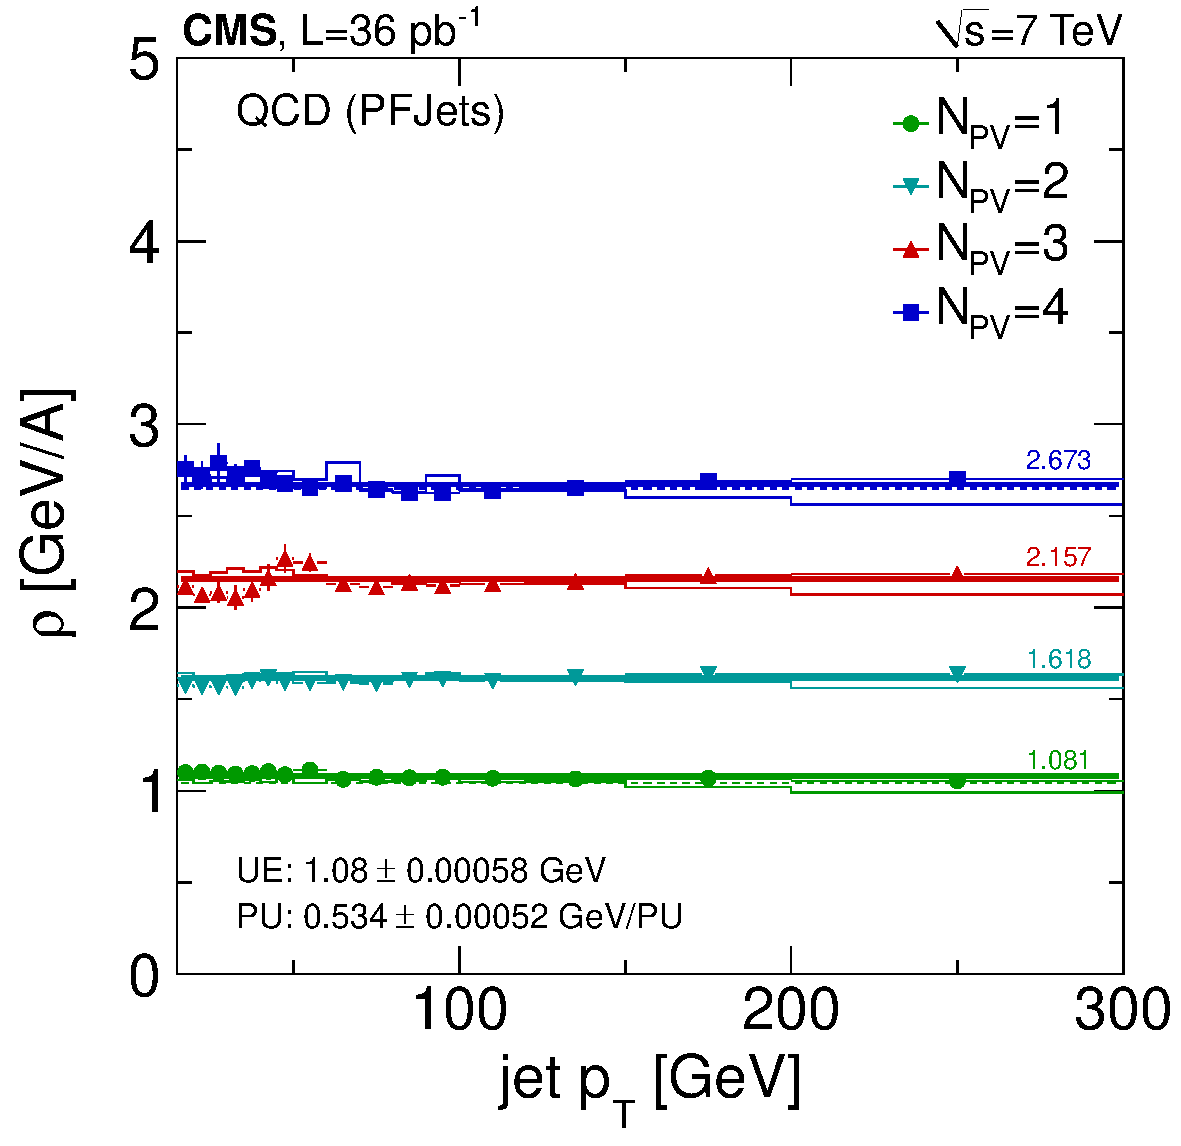
\includegraphics[width=0.45\textwidth]{Figures/JEC/QCD_RhoVsJet1Pt}
    \caption{Pile-up and underlying event PF \pt-density $\rho$, as a function of the leading jet \pt in the QCD multijet sample for various pile-up conditions (here $N_\text{PV}$ denotes the number of reconstructed vertices, and A denotes the unit area in the $y-\phi$ space).}
    \label{fig:fastjet}
  \end{center}
\end{figure}

\subsubsection{Average Offset Method}

The average offset method attempts to measure the average energy due to noise and pile-up, clustered inside the jet area, in addition to the energy associated with the jet shower itself. The measurement of the noise contribution is made in zero bias events by vetoing those that pass the minimum bias trigger. In the remaining events, the energy inside a cone of radius $R=0.5$ in the $\eta-\phi$ space is summed. The measurement is performed in cones centered at a specific $\eta$ bin and averaged across $\phi$. The noise contribution is found to be less than $250\MeV$ in \pt, over the entire $\eta$ range. The total average offset (over the entire dataset) is determined from inclusive zero bias events (with no veto on minimum bias triggers) and is classified according to the number of reconstructed vertices. Figure~\ref{fig:offset} shows the average offset \pt as a function of $\eta$ and for different pile-up conditions. The calorimetric offset \pt shows strong variations as a function of $\eta$, which follow the non-uniform particle response in the calorimeter, while for PF candidates, the offset \pt is more uniform versus $\eta$. The higher measured offset \pt for the PF-candidates is due to the much higher response with respect to the pure calorimetric objects. The observed $\eta$-asymmetry is related to calorimeter instrumental effects. For the highest number of vertices, in particular, the asymmetry is also of statistical nature (the adjacent points are highly correlated because at a given $\eta$ a large fraction of the energy in a cone of $R=0.5$ also ends up in overlapping cones). Figure~\ref{fig:PUcomposition} shows the breakdown, in terms of PF candidates, of the average offset \pt in events with one PU interaction, as measured in the data and compared to the MC prediction. The slight asymmetry observed in the MC is due to the asymmetric noise description in the specific version of the simulation. The average offset in \pt scales linearly with the number of reconstructed primary vertices, as shown in Fig.~\ref{fig:pileupPF}. The linear scaling allows the expression of the jet offset correction as follows:

\begin{equation}
  C_\text{offset}(\eta,\pt^{raw},N_\text{PV}) = 1-\frac{(N_\text{PV}-1)\cdot\mathcal{O}(\eta)}{\pt^{raw}},
\end{equation}

where $\mathcal{O}(\eta)$ is the average \pt due to one pile-up event, $\pt^{raw}$ is the \pt of the uncorrected jet, and $N_\text{PV}$ is the number of reconstructed primary vertices. The average offset method can be applied to jet algorithms that produce circular jets, while the quantity $\mathcal{O}(\eta)$ scales to larger cone sizes in proportion to the jet area. It should be noted that, in both the average offset subtraction and in the jet area method, the noise contribution and the UE are not subtracted. Because of the good description of the noise contribution in the simulation, the noise is taken into account with the MC-based correction.

\begin{figure}[ht!]
  \begin{center}
    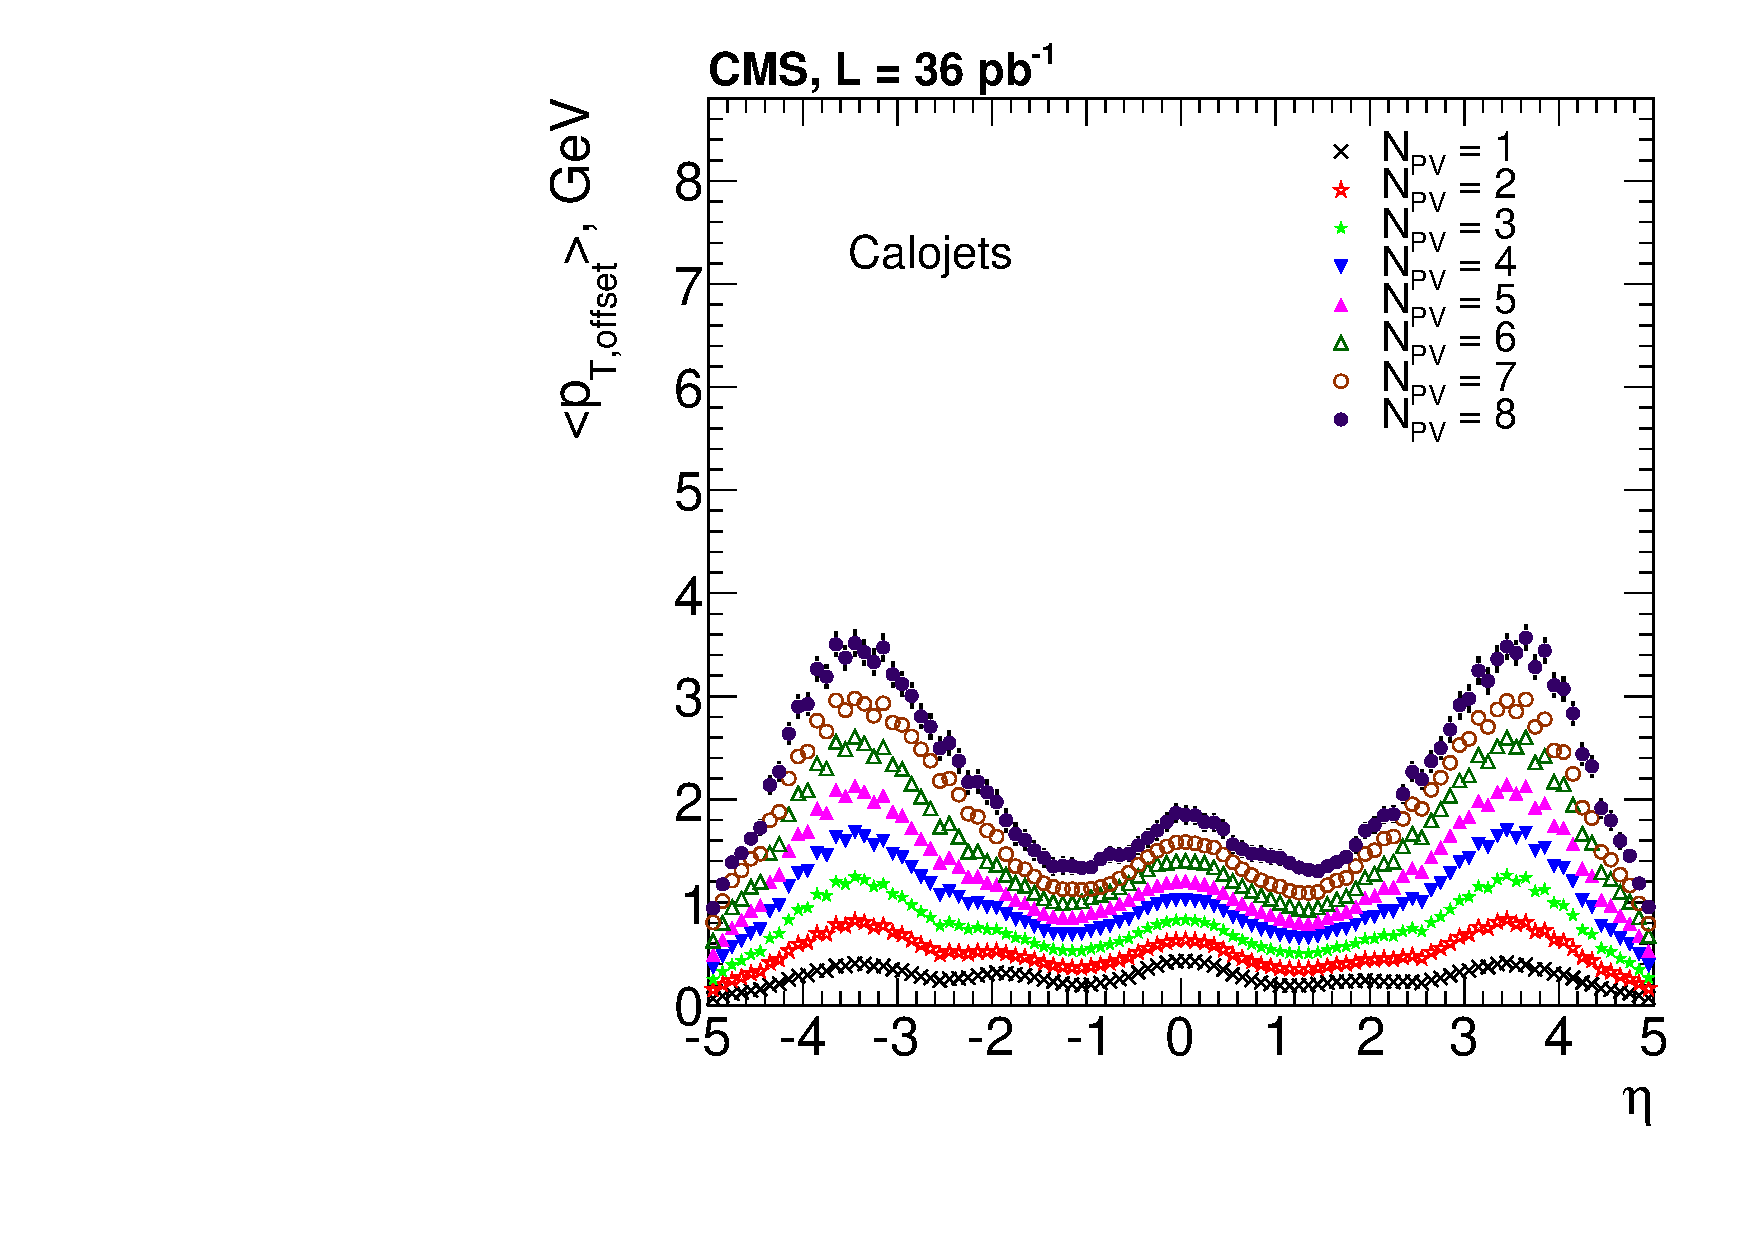
\includegraphics[width=0.45\textwidth]{Figures/JEC/p_AvgpTinC5_NoisePileup_PV_7TeV_run2010B_JNST}
    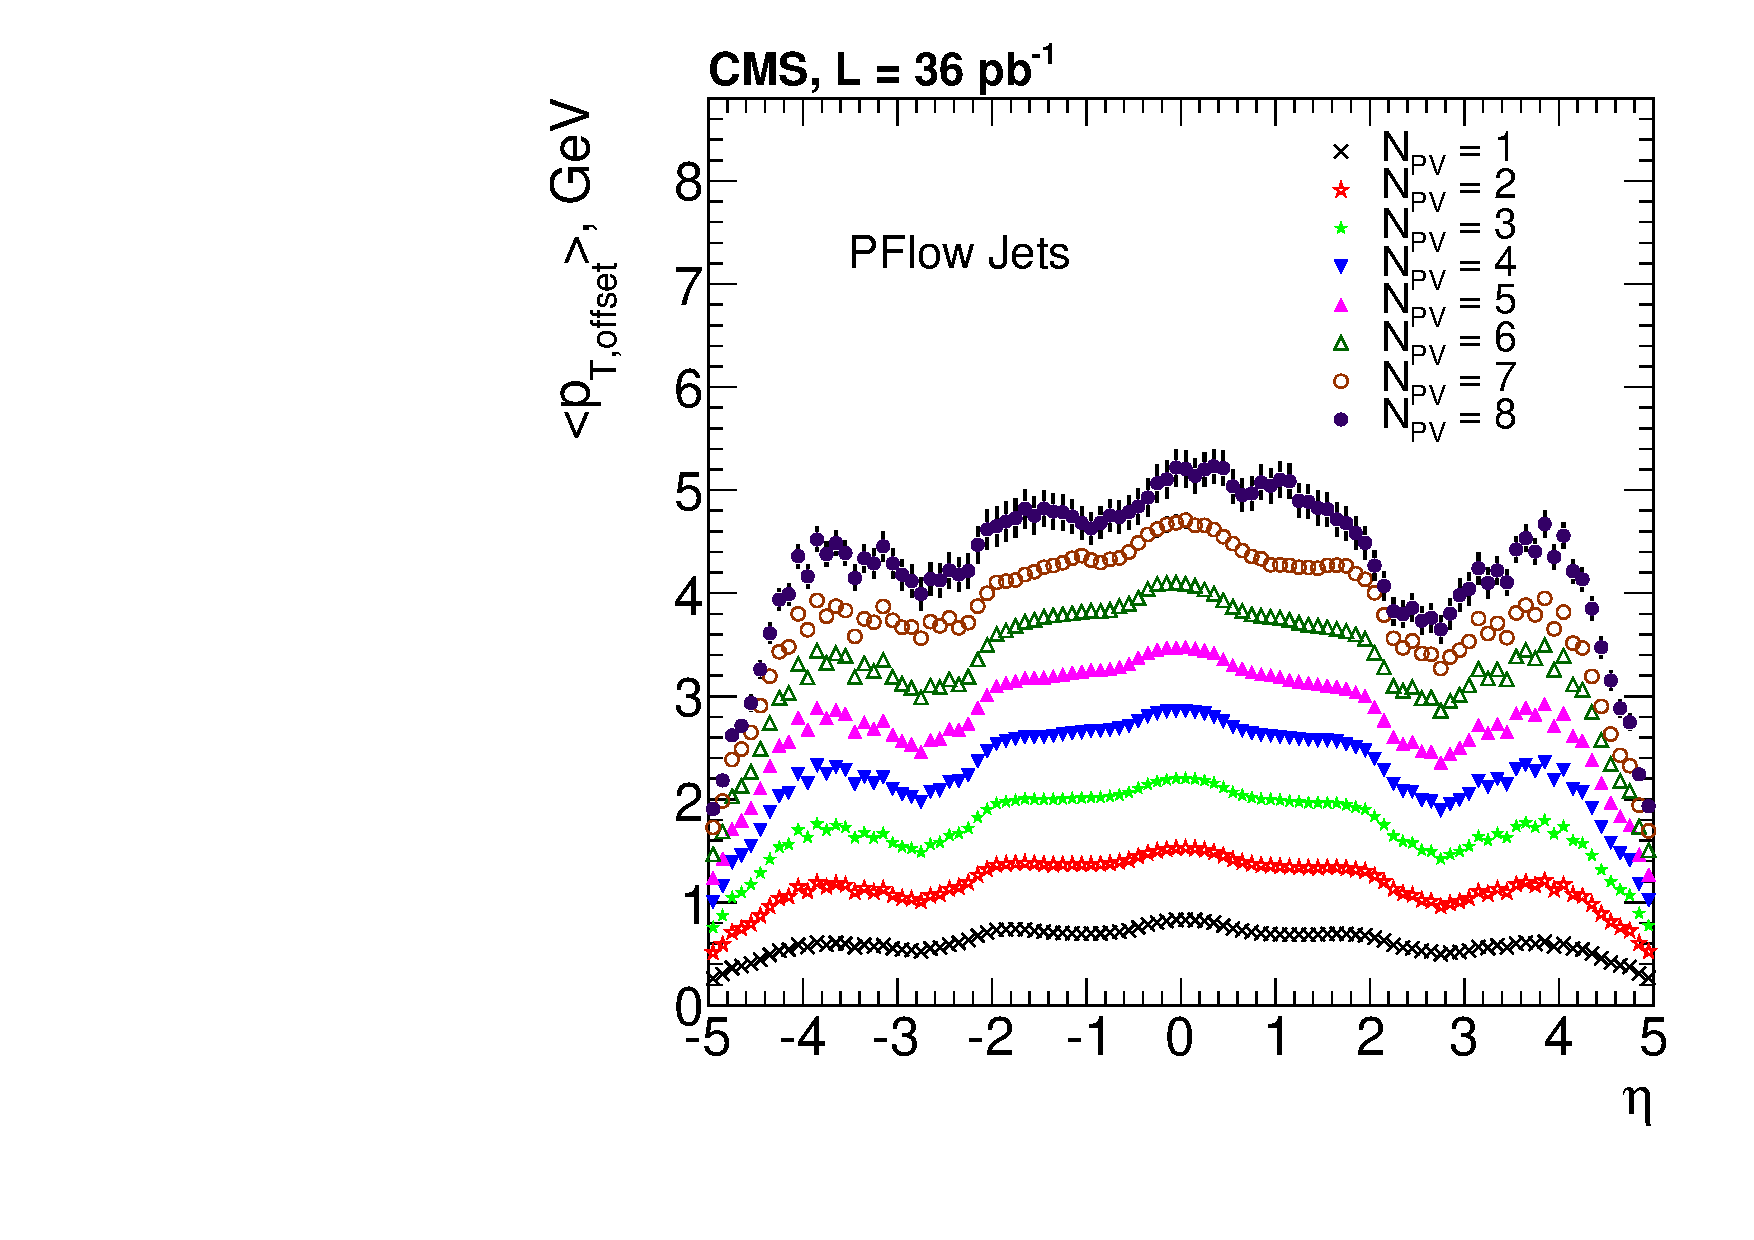
\includegraphics[width=0.45\textwidth]{Figures/JEC/p_AvgpTinPF5_NoisePileup_PV_7TeV_run2010B_JNST}
    \caption{Average offset in \pt, as a function of $\eta$, measured in minimum bias events for different pile-up conditions (categorized according to the number $N_\text{PV}$ of reconstructed primary vertices). Left: CALO jets. Right: PF jets.}
    \label{fig:offset}
  \end{center}
\end{figure}

\begin{figure}[ht!]
  \begin{center}
    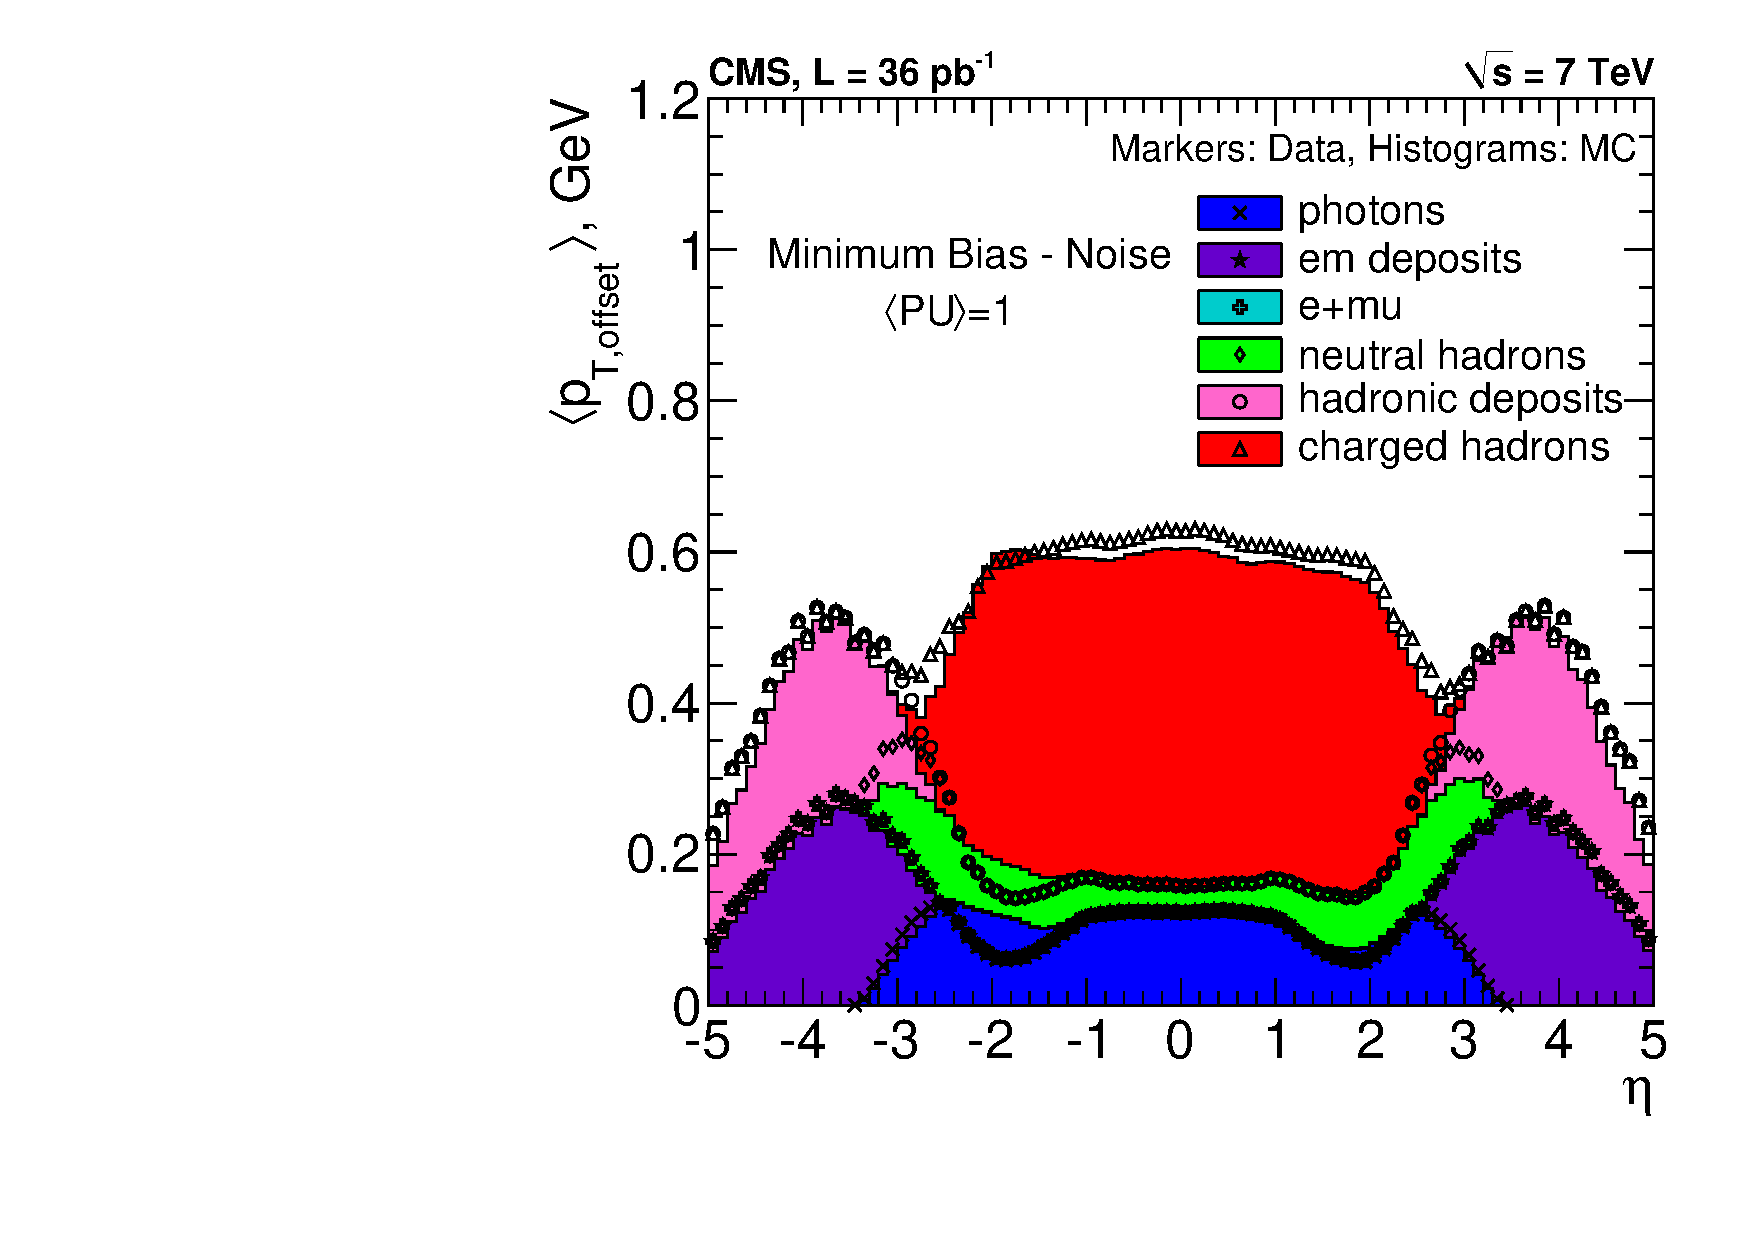
\includegraphics[width=0.45\textwidth]{Figures/JEC/h_AvgpTinPF5_stacked_MinBiasMinusZB}
    \caption{Breakdown of the average offset \pt, in terms of the PF candidates, as a function of $\eta$, for events with one PU interaction. Data are shown by markers and MC is shown as filled histograms.}
    \label{fig:PUcomposition}
  \end{center}
\end{figure}

\begin{figure}[ht!]
  \begin{center}
    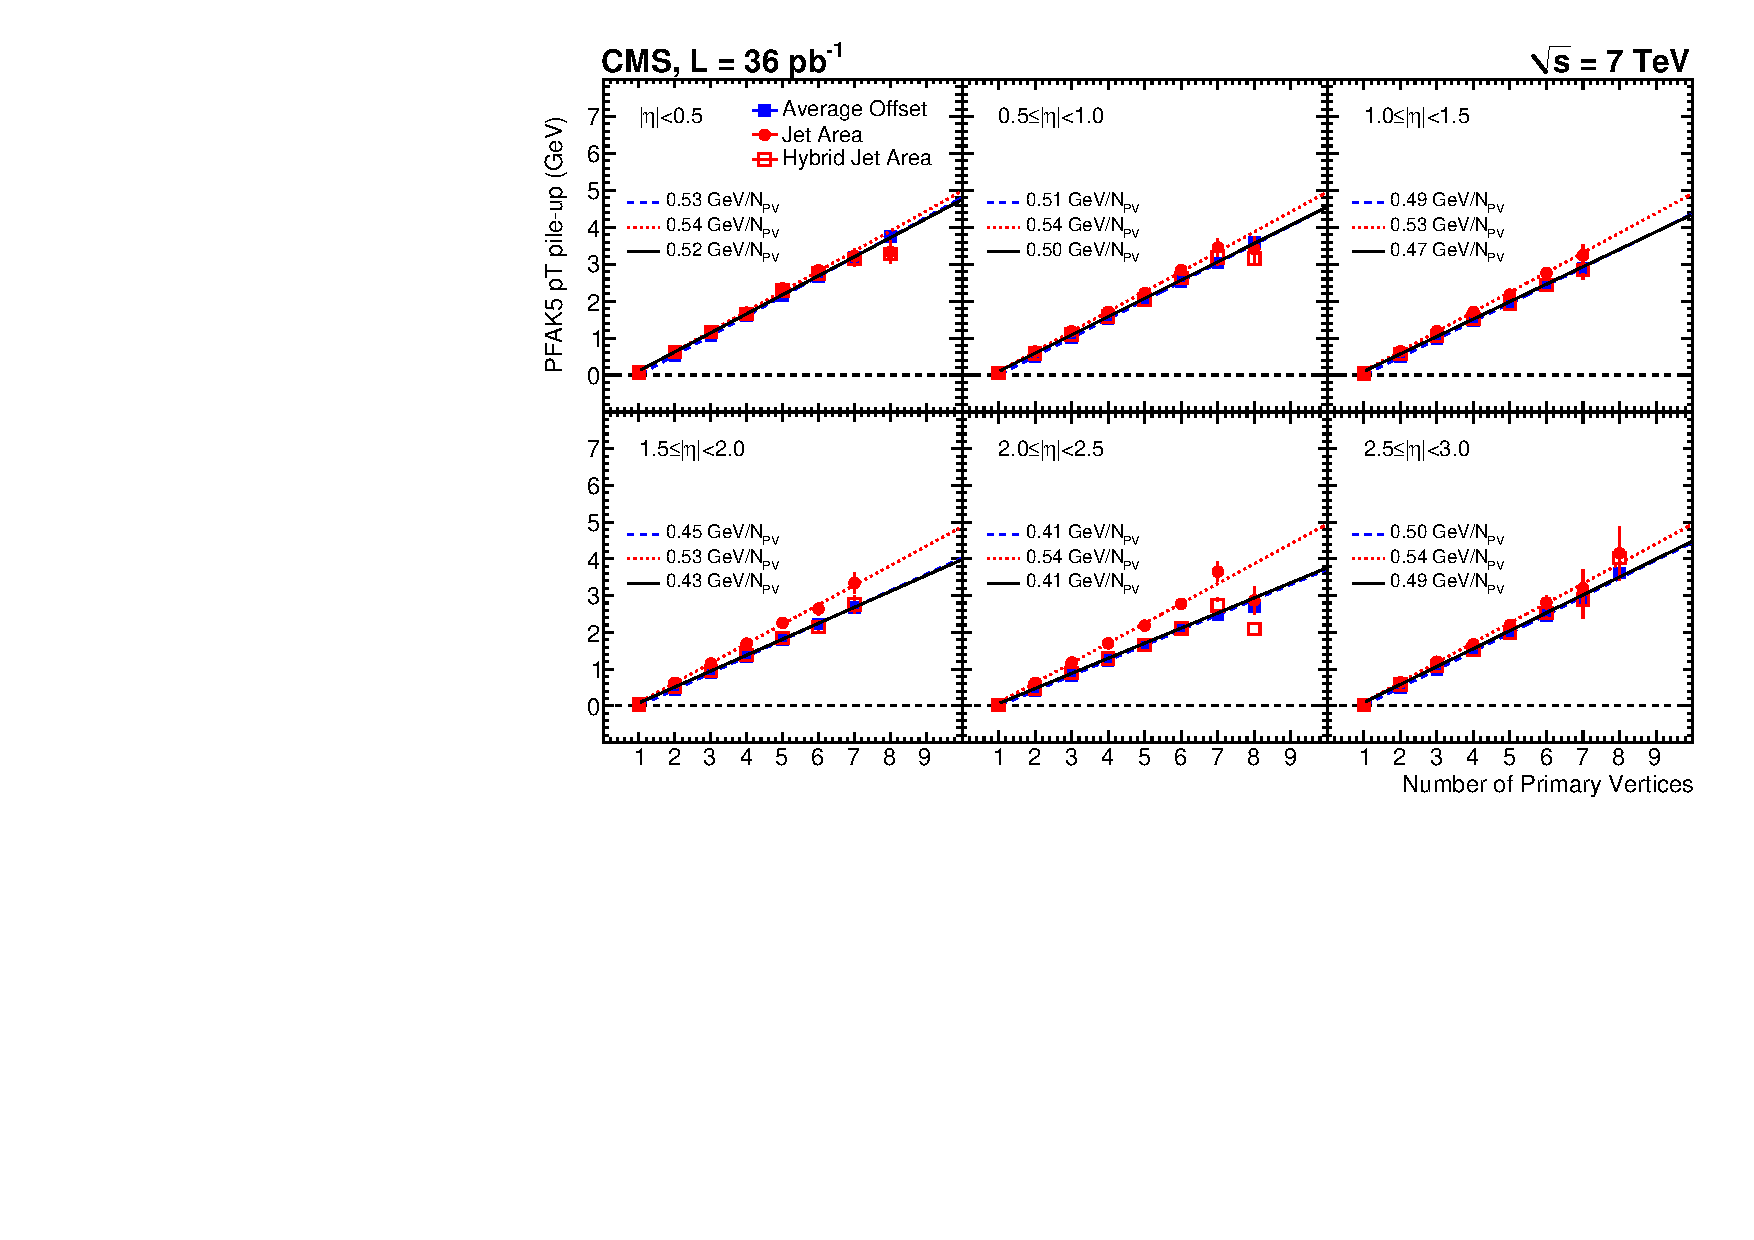
\includegraphics[width=0.9\textwidth]{Figures/JEC/PileUpComparison_NoPFNoPU_PF}
    \caption{Average PF jet pile-up \pt, as a function of the number of reconstructed vertices ($N_\text{PV}$) for the jet area, the average offset, and the hybrid jet area methods in 6 different $\eta$ regions. In the y-axis title, PFAK5 denotes the PF jets reconstructed with the anti-$k_T$ algorithm with distance parameter $R=0.5$.}
    \label{fig:pileupPF}
  \end{center}
\end{figure}

\subsubsection{Hybrid Jet Area Method}

The measurement of the average offset presented in the previous paragraph confirms the $\eta$-dependence of the offset energy. This is explained by the fact that the measured offset is the convolution of the pile-up activity with the detector response. In order to take into account the $\eta$-dependence, a hybrid jet area method is employed:

\begin{equation}
\label{eq:hybrid}
  C_\text{hybrid}(\pt^{raw},\eta,A_j,\rho) = 1-\frac{(\rho-\langle\rho_\text{UE}\rangle)\cdot\beta(\eta)\cdot A_j}{\pt^{raw}}.
\end{equation}

In Eq.~(\ref{eq:hybrid}), the \pt density $\rho$ and the corresponding density due to the UE, $\langle\rho_{UE}\rangle$ are constants over the entire $\eta$ range. The multiplicative factor $\beta(\eta)$ corrects for the non-uniformity of the energy response and is calculated from the modulation of the average offset in \pt (Fig.~\ref{fig:offset}).

In the case of PF jets, the response variation versus $\eta$ is relatively small and the hybrid jet area method is found to be in excellent agreement with the average offset method. Figure~\ref{fig:pileupPF} shows the average offset in \pt as a function of the number of reconstructed primary vertices, for the three different methods (jet area, average offset, hybrid jet area). It can be seen that the differences between the jet area method and the average offset method are entirely due to the response dependence on $\eta$. The hybrid jet area method is chosen for the pile-up correction of PF jets. In the case of CALO jets, and also JPT jets (initially reconstructed as CALO jets), the response variation versus $\eta$ shows dramatic changes and neither the simple jet area nor the hybrid jet area methods are able to reproduce the average offset measurement. Therefore, for CALO jets, the average offset method is the one chosen for the pile-up correction.

\subsubsection{Offset Uncertainty}\label{sec:offset_unc}

The uncertainty of the offset correction is quantified using the jet area method. Specifically, the quantities $\rho$ and $\langle\rho_\text{UE}\rangle$ in Eq.~(\ref{eq:fastjet}) are varied independently and the resulting shifts are added in quadrature. The event \pt-density $\rho$ uncertainty is estimated as $0.2\GeV$ per unit jet area and per pile-up event. This uncertainty is based on the maximum slope difference between the jet area and the average offset methods, and the residual non-closure in the average offset method. The UE \pt-density $\langle\rho_\text{UE}\rangle$ uncertainty is estimated as $0.15\GeV$ per unit jet area, based on the differences observed between the QCD multijet and Z+jets samples, and on the effective difference when applied in the inclusive jet cross-section measurement. Figure~\ref{fig:offsetUnc} shows the uncertainty of the offset correction, as a function of jet \pt and the number of primary vertices.

\begin{figure}[ht!]
  \begin{center}
    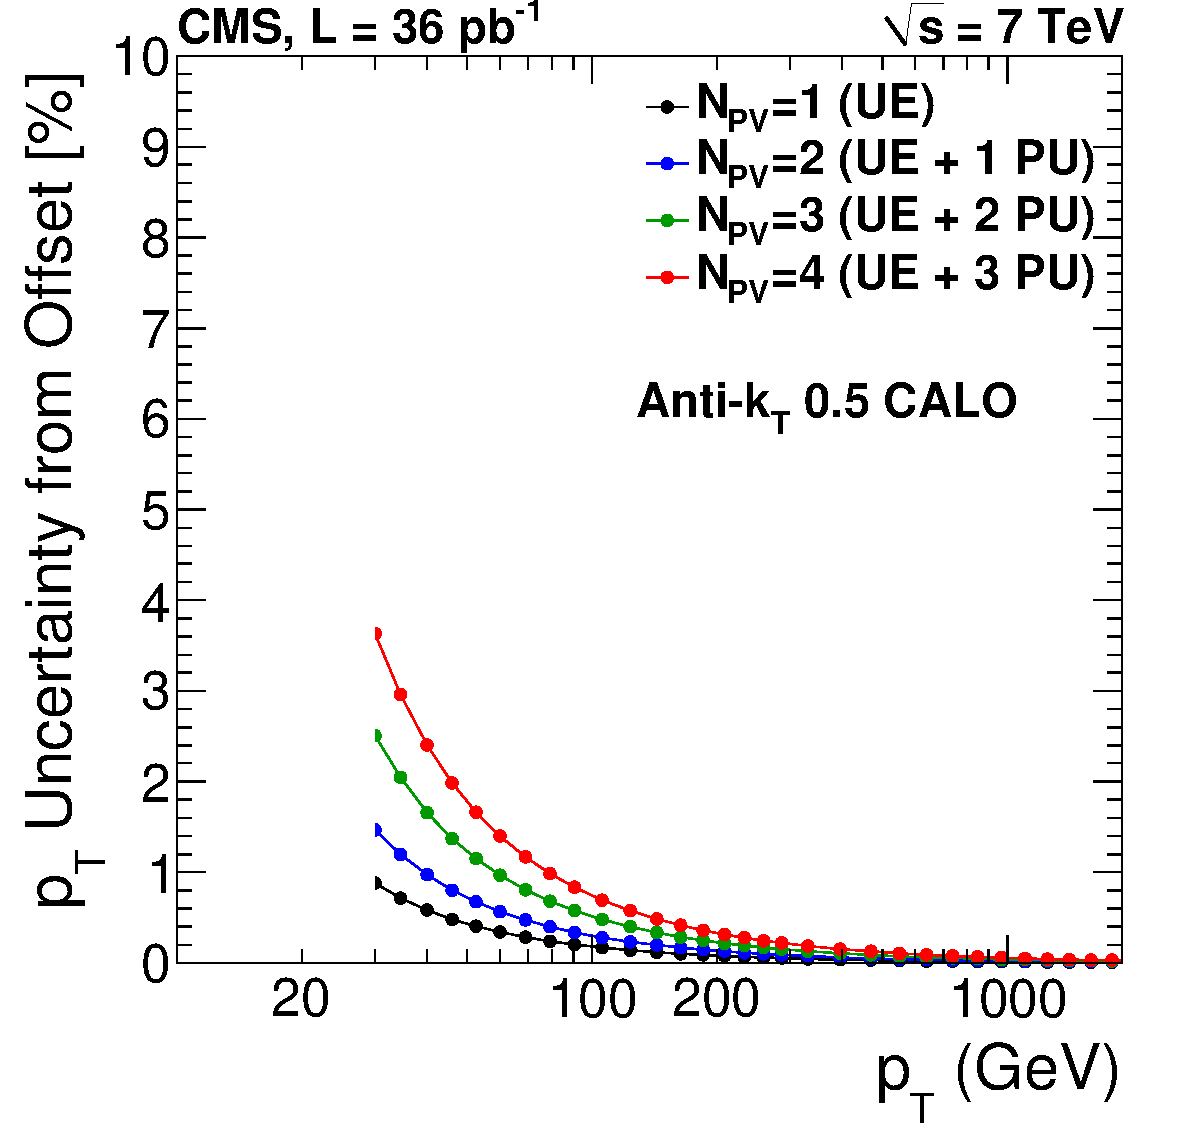
\includegraphics[width=0.45\textwidth]{Figures/JEC/JECUncert_Offset_CALOAK5.pdf}
    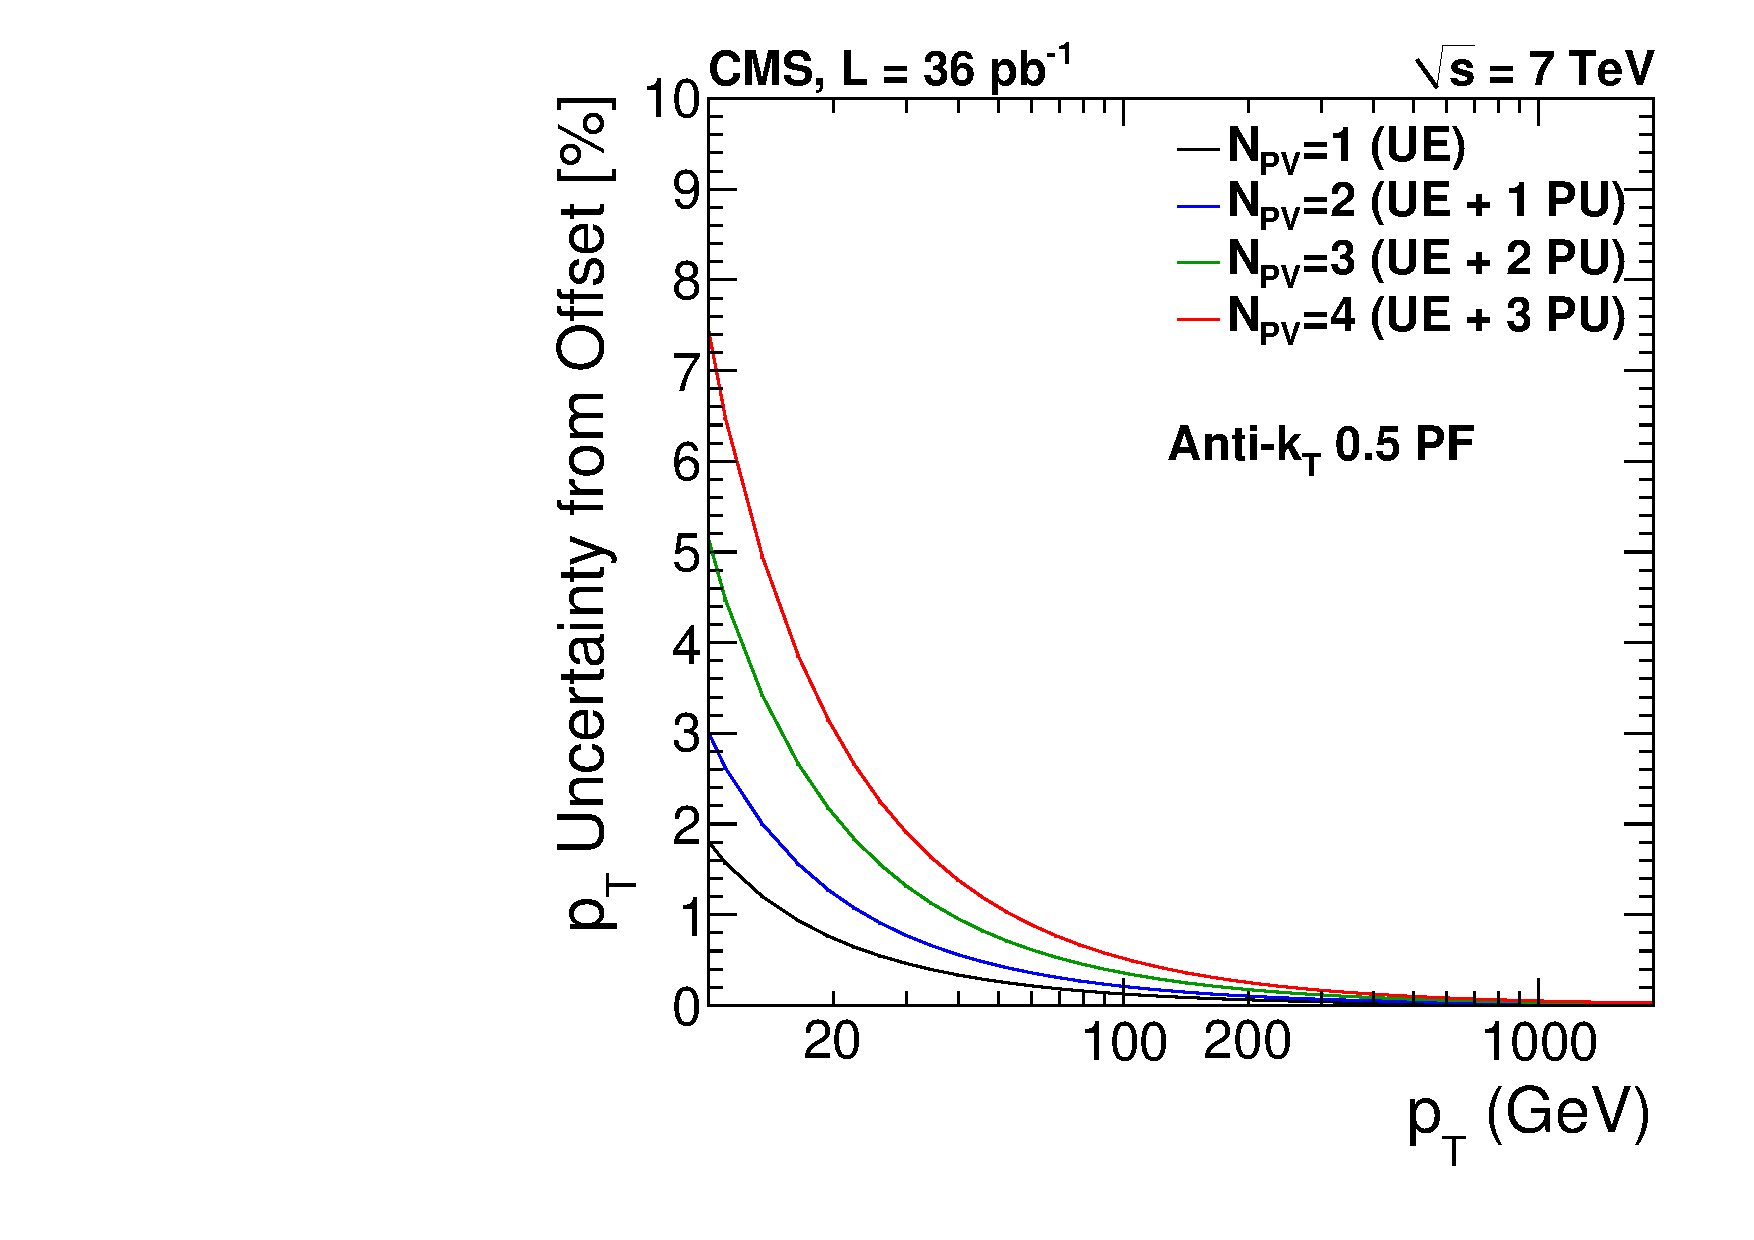
\includegraphics[width=0.45\textwidth]{Figures/JEC/JECUncert_Offset_PFAK5.pdf}
    \caption{Offset jet-energy-correction uncertainty as a function of jet \pt. Left: CALO jets. Right: PF jets.}
    \label{fig:offsetUnc}
  \end{center}
\end{figure}

